\chapter{Ánh xạ bảo giác và quy tắc tán xạ của dây mở}

\lectureoverview{Ánh xạ bảo giác trước hết xuất hiện như một đối xứng thực dụng của tĩnh điện học hai chiều. Tính khả vi phức biến đối xứng đó thành một đối xứng có thể tính toán được: các phương trình Cauchy--Riemann suy ra phương trình Laplace, và một đạo hàm phức độc lập với hướng sẽ bảo toàn các góc. Với bộ công cụ này, mặt thế giới của dây có thể được vẽ thành một dải, một nửa mặt phẳng, một hình trụ hoặc một đĩa mà không làm thay đổi vật lý. Khi đó, tán xạ dây mở trở thành một tích phân đường Gaussian trên đĩa với các xung lượng được chèn trên biên của nó, rồi tiếp theo là một tích phân trên các vị trí không tương đương của những chèn ấy.}

\section{Tĩnh điện học trong một thế giới hai chiều}

Ta bắt đầu với một bài toán tĩnh điện hai chiều theo đúng nghĩa đen. Các điện tích và những đường sức của chúng bị giới hạn trong một mặt phẳng; chúng không chỉ đơn thuần là các điện tích ba chiều thông thường mà chuyển động tình cờ nằm trong mặt phẳng. Khi đó định luật Gauss cho
\begin{equation}
  F(r)\propto \frac{1}{r},
  \qquad
  V(r)\propto \log r,
  \label{eq:l08-two-dimensional-coulomb}
\end{equation}
vì thông lượng đi qua một đường tròn có chu vi tăng theo \(r\).

Viết trường theo một thế vô hướng \(\phi\). Theo quy ước dấu dùng trên bảng,
\begin{equation}
  \mathbf E=\nabla\phi,
  \qquad
  \nabla\cdot\mathbf E=\rho,
\end{equation}
và do đó
\begin{equation}
  \nabla^2\phi
  =\frac{\partial^2\phi}{\partial x^2}
  +\frac{\partial^2\phi}{\partial y^2}
  =\rho.
  \label{eq:l08-poisson}
\end{equation}
Trong một miền không có điện tích, điều này rút gọn thành phương trình Laplace,
\begin{equation}
  \nabla^2\phi=0.
  \label{eq:l08-laplace-phi}
\end{equation}
\editorialnote{Nhiều giáo trình điện động lực học định nghĩa
\(\mathbf E=-\nabla\Phi\), khi đó
\(\nabla^2\Phi=-\rho\) sau khi hấp thụ các hằng số. Bài giảng dùng dấu thế ngược lại. Phương trình không nguồn và toàn bộ các lập luận bảo giác đều không thay đổi.}

\begin{figure}[H]
  \centering
  \includegraphics[width=0.72\textwidth]{lecture_08_figure_01.png}
  \caption{Các phương trình tĩnh điện được triển khai thành toán tử Poisson hai chiều.}
  \lectureframe{00:03:48}
  \label{fig:l08-electrostatics-board}
\end{figure}

Dấu cộng giữa hai đạo hàm không gian là điều quan trọng. Nó khiến đây là một phương trình elliptic chứ không phải một phương trình sóng. Các phép biến đổi bảo giác bảo toàn dạng không nguồn của nó, nên một nghiệm trên một miền có thể được chuyển sang một miền có hình dạng khác cùng với các điều kiện biên của nó. Điều này hữu ích trong tĩnh điện học, dòng chảy chất lưu hai chiều và bản đồ học trước khi hữu ích trong lý thuyết dây.

\begin{classroomqa}
\audiencequestion{Nếu toán tử Laplace triệt tiêu, đây có phải là một phương trình sóng dừng không? \lecturetimestamp{00:05:35}}
\lecturerresponse{Không. Cả hai đạo hàm không gian đều có cùng dấu và không có đạo hàm theo thời gian. Một phương trình sóng đòi hỏi sự phụ thuộc thời gian với dấu tương đối Lorentzian. Tĩnh điện học là tĩnh chính vì không có gì, kể cả sóng, đang biến thiên.}
\end{classroomqa}

\begin{classroomqa}
\audiencequestion{Có xoáy trong hai chiều không?
\lecturetimestamp{00:06:06}}
\lecturerresponse{Có, nhưng nó chỉ có một thành phần độc lập. Với
\(\mathbf E=(E_x,E_y)\),
\[
  \operatorname{curl}_{2d}\mathbf E
  =\partial_yE_x-\partial_xE_y.
\]
Có thể hình dung nó như thành phần vuông góc với bảng, mặc dù một thế giới nội tại hai chiều không cần một phương vuông góc bên ngoài như vậy. Trong số chiều cao hơn, đối tượng tương ứng một cách tự nhiên là một 2-dạng phản đối xứng.}
\end{classroomqa}

\section{Một đạo hàm không có hướng ưu tiên}

Đưa vào các tọa độ phức trên mặt phẳng gốc và mặt phẳng ảnh:
\begin{equation}
  z=x+iy,
  \qquad
  w=u+iv,
  \qquad
  w=w(z).
  \label{eq:l08-complex-coordinates}
\end{equation}
Ở đây \(x,y,u,v\) là các số thực. Xét cục bộ, đạo hàm phải là
\begin{equation}
  \frac{dw}{dz}
  =\lim_{\Delta z\to0}\frac{\Delta w}{\Delta z}.
  \label{eq:l08-complex-derivative}
\end{equation}
Mặt phẳng phức, khác với trục thực, cho phép vô số hướng tiến tới. Một ánh xạ liên tục và trơn theo nghĩa thông thường không nhất thiết cho cùng một tỉ số theo mọi hướng.

Hãy so sánh hai cách tiến tới đơn giản. Dọc theo hướng \(x\), \(dy=0\), nên
\begin{equation}
  \left.\frac{dw}{dz}\right|_x
  =\frac{\partial u}{\partial x}
  +i\frac{\partial v}{\partial x}.
\end{equation}
Dọc theo hướng \(y\), \(dx=0\), và
\begin{equation}
  \left.\frac{dw}{dz}\right|_y
  =\frac{1}{i}\frac{\partial u}{\partial y}
  +\frac{\partial v}{\partial y}
  =\frac{\partial v}{\partial y}
  -i\frac{\partial u}{\partial y}.
\end{equation}
Việc đồng nhất phần thực và phần ảo cho
\begin{equation}
  \boxed{
  \frac{\partial u}{\partial x}
  =\frac{\partial v}{\partial y},
  \qquad
  \frac{\partial u}{\partial y}
  =-\frac{\partial v}{\partial x}}
  \label{eq:l08-cauchy-riemann}
\end{equation}
Đây là các phương trình Cauchy--Riemann. Dưới những giả thiết khả vi thông thường, chúng cũng đủ để giới hạn
\eqref{eq:l08-complex-derivative} độc lập với hướng. Một hàm có tính chất này là giải tích, hay chỉnh hình, tại điểm đó.

\begin{figure}[H]
  \centering
  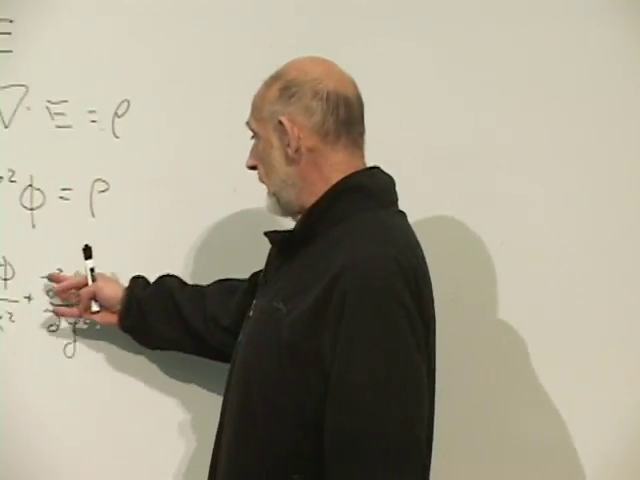
\includegraphics[width=0.70\textwidth]{lecture_08_figure_02.png}
  \caption{Cặp phương trình Cauchy--Riemann hoàn chỉnh, kể cả dấu trừ tương đối.}
  \lectureframe{00:19:48}
  \label{fig:l08-cr-board}
\end{figure}

Bài giảng phân biệt ngắn gọn các thuật ngữ liên quan. Một hàm chỉnh hình trên toàn bộ mặt phẳng phức hữu hạn là một hàm nguyên. Một hàm phân hình có thể có các cực cô lập. Vì vậy \(1/z\) là giải tích ở ngoài \(z=0\), nhưng nó không phải là hàm nguyên.

\section{Các hàm điều hòa liên hợp và hình học bảo giác}

Các phương trình Cauchy--Riemann là các phương trình bậc một ghép cặp, nhưng chúng kéo theo các phương trình bậc hai riêng rẽ. Lấy đạo hàm của
\(\partial_xu=\partial_yv\) theo \(x\), lấy đạo hàm của
\(\partial_yu=-\partial_xv\) theo \(y\), rồi cộng lại:
\begin{align}
  \partial_x^2u&=\partial_x\partial_yv,\\
  \partial_y^2u&=-\partial_y\partial_xv,\\
  \therefore\qquad
  \partial_x^2u+\partial_y^2u&=0.
  \label{eq:l08-harmonic-u}
\end{align}
Lặp lại lập luận với \(u\) và \(v\) hoán đổi cho nhau thì được
\begin{equation}
  \partial_x^2v+\partial_y^2v=0.
  \label{eq:l08-harmonic-v}
\end{equation}
Vì thế phần thực và phần ảo của một hàm giải tích là các hàm điều hòa liên hợp. Hai hàm điều hòa tùy ý không tự động tạo thành một hàm giải tích; chúng vẫn phải được liên hệ với nhau bởi
\eqref{eq:l08-cauchy-riemann}.

\begin{figure}[H]
  \centering
  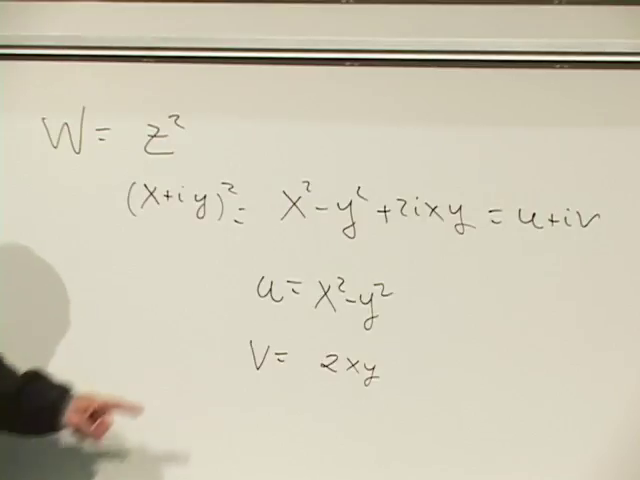
\includegraphics[width=0.68\textwidth]{lecture_08_figure_03.png}
  \caption{Các đạo hàm hỗn hợp triệt tiêu, để lại phương trình Laplace cho một thành phần của ánh xạ giải tích.}
  \lectureframe{00:23:09}
  \label{fig:l08-harmonic-board}
\end{figure}

Cũng có một cách diễn giải vectơ hữu ích. Nếu
\(\mathbf F=(u,-v)\), thì hai phương trình Cauchy--Riemann phát biểu, tùy theo quy ước định hướng đã chọn, rằng cả phân kỳ lẫn xoáy hai chiều của \(\mathbf F\) đều triệt tiêu. Đây là sự quay lại với tĩnh điện học đã được báo trước.

\subsection{Vì sao các góc được bảo toàn}

Viết hai độ dời phức nhỏ ở dạng cực:
\begin{equation}
  \delta z=\rho e^{i\theta},
  \qquad
  \Delta z=\rho'e^{i\theta'}.
\end{equation}
Tỉ số của chúng có pha \(\theta-\theta'\), đúng bằng góc giữa chúng.
Dưới một ánh xạ giải tích,
\begin{equation}
  \frac{\delta w}{\delta z}
  =\frac{\Delta w}{\Delta z}
  =w'(z),
\end{equation}
vì đạo hàm không phụ thuộc vào hướng. Sắp xếp lại cho
\begin{equation}
  \frac{\Delta z}{\delta z}
  =\frac{\Delta w}{\delta w}.
  \label{eq:l08-angle-ratio}
\end{equation}
Hai vế có cùng pha, nên góc giữa các độ dời ban đầu bằng góc giữa các ảnh của chúng.

\begin{figure}[H]
  \centering
  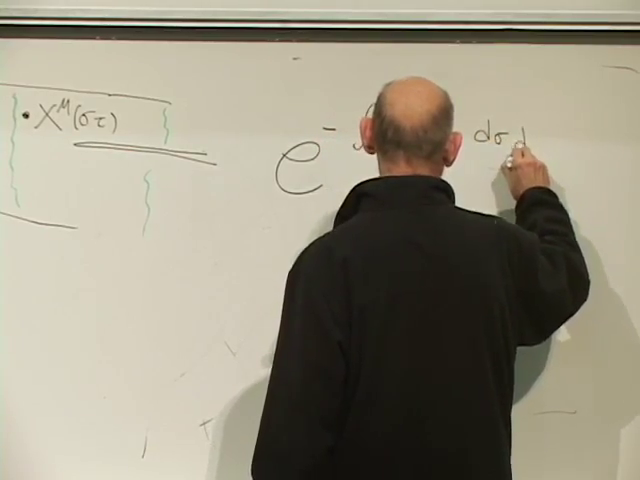
\includegraphics[width=0.70\textwidth]{lecture_08_figure_04.png}
  \medskip

  \begin{tikzpicture}[x=0.9cm,y=0.9cm,>=Latex]
    \begin{scope}
      \draw[->] (-0.2,0) -- (2.3,0);
      \draw[->] (0,-0.2) -- (0,2.1);
      \draw[very thick,blue!65!black,->] (0,0) -- (1.85,0.45)
        node[right] {\(\delta z\)};
      \draw[very thick,orange!75!black,->] (0,0) -- (0.72,1.65)
        node[above] {\(\Delta z\)};
      \draw (0.58,0.14) arc[start angle=14,end angle=66,radius=0.60];
      \node at (1.0,-0.55) {\(z\)-plane};
    \end{scope}
    \draw[->,thick] (3.0,0.9) -- (4.2,0.9)
      node[midway,above] {\(w(z)\)};
    \begin{scope}[xshift=5.0cm]
      \draw[->] (-0.2,0) -- (2.3,0);
      \draw[->] (0,-0.2) -- (0,2.1);
      \draw[very thick,blue!65!black,->] (0,0) -- (1.65,0.70)
        node[right] {\(\delta w\)};
      \draw[very thick,orange!75!black,->] (0,0) -- (0.48,1.62)
        node[above] {\(\Delta w\)};
      \draw (0.54,0.23) arc[start angle=23,end angle=74,radius=0.59];
      \node at (1.0,-0.55) {\(w\)-plane};
    \end{scope}
  \end{tikzpicture}
  \caption{Chứng minh trên bảng và một cách dựng lại cục bộ gọn gàng. Phép nhân với \(w'(z)\) quay và co giãn mọi hướng vi phân theo cùng một lượng, nhờ đó bảo toàn góc tương đối của chúng.}
  \lectureframe{00:34:11}
  \label{fig:l08-angle-proof}
\end{figure}

Lập luận cục bộ này giả sử \(w'(z)\neq0\). Tại một điểm tới hạn, ánh xạ có thể không còn là một-một theo địa phương, và khi đó phải xét riêng hình học. Tránh xa những điểm như vậy, các ánh xạ giải tích và các ánh xạ bảo giác bảo toàn định hướng là cùng một đối tượng xét theo địa phương.

\section{Những ví dụ để luyện mắt}

\subsection{Phép bình phương và liên hợp phức}

Với \(w=z^2\),
\begin{equation}
  (x+iy)^2=x^2-y^2+2ixy=u+iv,
\end{equation}
nên
\begin{equation}
  u=x^2-y^2,
  \qquad
  v=2xy.
  \label{eq:l08-z-squared-components}
\end{equation}
Các đạo hàm bậc hai của \(u\) là \(2\) và \(-2\); các đạo hàm bậc hai của \(v\) thì riêng rẽ đều triệt tiêu. Cả hai đều điều hòa, và việc vi phân trực tiếp cũng xác nhận các phương trình Cauchy--Riemann.

\begin{figure}[H]
  \centering
  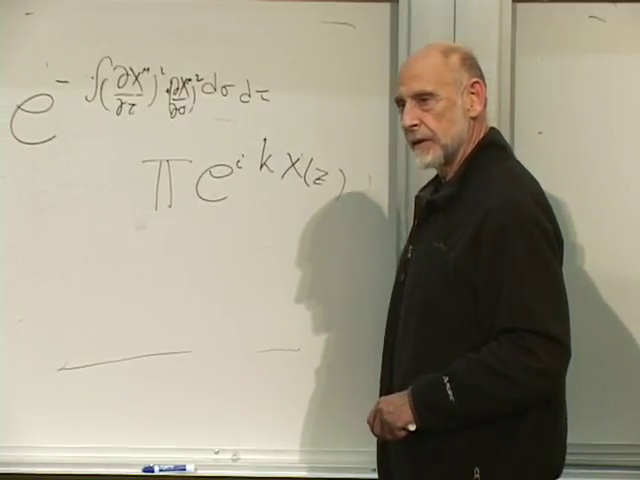
\includegraphics[width=0.72\textwidth]{lecture_08_figure_05.png}
  \caption{Ánh xạ bình phương được tách thành các thành phần điều hòa thực và ảo của nó.}
  \lectureframe{00:36:45}
  \label{fig:l08-z-square-board}
\end{figure}

\begin{classroomqa}
\audiencequestion{Liệu \(1/z\) có cho một ví dụ không giải tích không?
\lecturetimestamp{00:37:49}}
\lecturerresponse{Chỉ tại một điểm. Nó giải tích ở mọi nơi \(z\neq0\)
và có một cực tại gốc tọa độ. Muốn thấy một ánh xạ thất bại phép kiểm tra
Cauchy--Riemann ở mọi nơi, liên hợp phức là một ví dụ tốt hơn.}
\end{classroomqa}

Ngược lại,
\begin{equation}
  w=\bar z=x-iy
  \qquad\Longrightarrow\qquad
  u=x,\quad v=-y
\end{equation}
đảo ngược định hướng. Các đạo hàm của nó không thỏa phương trình
Cauchy--Riemann thứ nhất do sai khác dấu, nên nó không giải tích như một hàm của
\(z\).

\begin{figure}[H]
  \centering
  \includegraphics[width=0.62\textwidth]{lecture_08_figure_06.png}
  \caption{Liên hợp phức cung cấp một phản ví dụ cố ý không giải tích.}
  \lectureframe{00:38:38}
  \label{fig:l08-conjugate-board}
\end{figure}

\subsection{Hàm mũ và hàm nghịch đảo của nó}

\begin{classroomqa}
\audiencequestion{Nếu \(e^z\) là giải tích, vì sao hàm nghịch đảo của nó
\(\log z\) cũng phải giải tích? \lecturetimestamp{00:40:38}}
\lecturerresponse{Ở nơi hàm nghịch đảo tồn tại và \(w'(z)\neq0\), đạo hàm của nó là \(1/w'(z)\). Vì thế tính độc lập với hướng được bảo toàn. Trên toàn cục, logarit là đa trị, nên ta chọn một nhánh và loại trừ điểm phân nhánh cùng đường cắt của nó. Mệnh đề bảo giác cục bộ vẫn đúng trên miền đã chọn đó.}
\end{classroomqa}

Công thức Euler cho
\begin{equation}
  w=e^z=e^{x+iy}
  =e^x(\cos y+i\sin y),
\end{equation}
do đó
\begin{equation}
  u=e^x\cos y,
  \qquad
  v=e^x\sin y.
  \label{eq:l08-exponential-components}
\end{equation}
Chẳng hạn,
\(\partial_xu=e^x\cos y=\partial_yv\), và phương trình Cauchy--Riemann thứ hai cũng theo ra trực tiếp như vậy.

\begin{figure}[H]
  \centering
  \includegraphics[width=0.68\textwidth]{lecture_08_figure_07.png}
  \caption{Các thành phần thực và ảo của ánh xạ mũ.}
  \lectureframe{00:42:23}
  \label{fig:l08-exponential-board}
\end{figure}

\section{Nửa mặt phẳng, dải, hình trụ và đĩa}

\subsection{Logarit biến bán kính thành thời gian}

Xét nửa mặt phẳng phải, nơi
\(-\pi/2<\theta<\pi/2\), và viết
\begin{equation}
  z=re^{i\theta},
  \qquad
  w=\log z=\log r+i\theta.
  \label{eq:l08-log-map}
\end{equation}
Nửa mặt phẳng được ánh xạ thành dải vô hạn
\begin{equation}
  -\frac{\pi}{2}<\operatorname{Im}w<\frac{\pi}{2}.
\end{equation}
Các tia có \(\theta\) cố định trở thành các đường nằm ngang, còn các nửa đường tròn có \(r\) cố định trở thành các đường thẳng đứng. Gốc tọa độ được ánh xạ tới
\(\operatorname{Re}w=-\infty\), còn \(r=\infty\) tới
\(\operatorname{Re}w=+\infty\).

\begin{figure}[H]
  \centering
  \includegraphics[width=0.75\textwidth]{lecture_08_figure_08.png}
  \caption{Logarit biến nửa mặt phẳng phải thành một dải vô hạn: các tia cực và các nửa đường tròn trở thành một lưới chữ nhật trực giao.}
  \lectureframe{00:47:48}
  \label{fig:l08-log-strip-board}
\end{figure}

Dải là mặt thế giới chuẩn của một dây mở. Tọa độ bị chặn của nó là tham số dọc theo dây, còn phép tịnh tiến theo hướng không bị chặn tương ứng với thời gian mặt thế giới. Dưới ánh xạ mũ nghịch, một phép tịnh tiến theo thời gian trở thành một phép co giãn \(z\mapsto e^a z\). Vì vậy cùng một đối xứng trông như phép tịnh tiến trên dải và như sự dãn đều trên nửa mặt phẳng.

\begin{classroomqa}
\audiencequestion{Một giá trị cụ thể như \(r=1\) đi tới đâu, và các tọa độ trên dải có còn là tọa độ cực không? \lecturetimestamp{00:50:58}}
\lecturerresponse{Một đường tròn có bán kính cố định trở thành một đường thẳng đứng tại
\(\operatorname{Re}w=\log r\); riêng \(r=1\) được ánh xạ tới đường trung tâm
\(\operatorname{Re}w=0\). Tọa độ cực mô tả mặt phẳng
\(z\). Mặt phẳng \(w\) dùng các tọa độ chữ nhật thông thường
\((\log r,\theta)\).}
\end{classroomqa}

Nếu toàn bộ mặt phẳng bị đục lỗ được ánh xạ bởi \(\log z\), tọa độ góc có chu kỳ \(2\pi\). Vì vậy dải thu được có các cạnh trên và dưới được đồng nhất với nhau: nó là một hình trụ vô hạn. Nửa mặt phẳng có biên mô tả mặt thế giới của dây mở; toàn mặt phẳng, không có biên và có góc tuần hoàn, mô tả một hình trụ của dây kín.

\begin{figure}[H]
  \centering
  \includegraphics[width=0.75\textwidth]{lecture_08_figure_09.png}
  \caption{Bức tranh nửa mặt phẳng/dải và phép đồng nhất tuần hoàn biến toàn bộ mặt phẳng bị đục lỗ thành một hình trụ của dây kín.}
  \lectureframe{00:54:23}
  \label{fig:l08-open-closed-board}
\end{figure}

\subsection{Một ánh xạ Cayley tới đĩa đơn vị}

Một ánh xạ phân tuyến tính, hay Möbius, biến nửa mặt phẳng phải thành đĩa đơn vị:
\begin{equation}
  w=\frac{z-1}{z+1}.
  \label{eq:l08-cayley}
\end{equation}
Nó biến \(z=0\) thành \(-1\), \(z=\infty\) thành \(+1\), và trục ảo thành \(|w|=1\). Nếu \(z=ir\),
\begin{equation}
  \left|\frac{ir-1}{ir+1}\right|=1.
\end{equation}
Các điểm thỏa \(\operatorname{Re}z>0\) nằm bên trong đường tròn; nửa mặt phẳng trái được ánh xạ ra bên ngoài nó.
\editorialnote{Trong quá trình suy dẫn trực tiếp, nghịch đảo
\((z+1)/(z-1)\) được viết ra trong khi ảnh là miền trong của đĩa đang được mô tả.
Nghịch đảo đó có cùng biên là đường tròn đơn vị nhưng biến nửa mặt phẳng phải ra miền ngoài. Phương trình \eqref{eq:l08-cayley} là quy ước cho miền trong đĩa, nhất quán với hình học đã nêu.}

\begin{figure}[H]
  \centering
  \includegraphics[width=0.72\textwidth]{lecture_08_figure_10.png}
  \caption{Phép dựng biên đường tròn đơn vị bằng ánh xạ phân tuyến tính. Quy ước nghịch đảo nhìn thấy trên bảng hoán đổi miền trong và miền ngoài.}
  \lectureframe{00:58:38}
  \label{fig:l08-cayley-board}
\end{figure}

Ánh xạ Möbius biến họ suy rộng gồm các đường tròn và đường thẳng thành các đường tròn và đường thẳng. Vì thế lưới gồm các tia và các đường tròn trên nửa mặt phẳng trở thành hai họ cung trực giao trên đĩa. Một đường kính thẳng đơn giản là trường hợp giới hạn của một đường tròn có tâm đi ra vô cực.

\begin{classroomqa}
\audiencequestion{Các cung được vẽ bên trong đĩa có thực sự là các đường tròn không?
\lecturetimestamp{01:00:55}}
\lecturerresponse{Có. Tâm của chúng nằm ở các vị trí khác nhau, thường ở ngoài phần đĩa nhìn thấy. Đường kính là giới hạn bán kính vô hạn của cùng họ đó.}
\end{classroomqa}

\begin{classroomqa}
\audiencequestion{Hình vẽ đĩa này có nghĩa là đó là một mặt cầu không, và nửa mặt phẳng còn lại đi đâu? \lecturetimestamp{01:01:21}}
\lecturerresponse{Hình vẽ ở đây là một đĩa phẳng, không phải mặt cầu. Nửa mặt phẳng phải được ánh xạ vào bên trong biên của nó, còn nửa mặt phẳng trái được ánh xạ ra bên ngoài. Nếu thêm điểm ở vô cực vào toàn bộ mặt phẳng phức, thì mặt phẳng mở rộng đó có thể được biểu diễn như một mặt cầu bằng phép chiếu lập thể; đó là một phát biểu toàn cục khác.}
\end{classroomqa}

\begin{classroomqa}
\audiencequestion{Những đường cong nào trên đĩa tương ứng với các tia xuyên tâm ban đầu và các nửa đường tròn bán kính không đổi? \lecturetimestamp{01:02:59}}
\lecturerresponse{Trục thực dương trở thành đường kính nối \(-1\) và \(+1\). Các tia khác trở thành những cung tròn nối cùng hai điểm biên đó. Các nửa đường tròn có bán kính cố định trở thành họ trực giao bắt đầu và kết thúc trên đường tròn đơn vị.}
\end{classroomqa}

\begin{figure}[H]
  \centering
  \includegraphics[width=0.72\textwidth]{lecture_08_figure_11.png}
  \caption{Các đường thẳng và nửa đường tròn trong nửa mặt phẳng trở thành các họ đường tròn và đường thẳng trực giao trong đĩa.}
  \lectureframe{01:03:48}
  \label{fig:l08-circle-grid-board}
\end{figure}

\section{Mặt thế giới của bốn dây}

Giờ ta có thể quay lại tán xạ. Hai dây mở đi vào, nhập lại thành một dây, truyền trong một khoảng thời gian tùy ý, rồi tách thành hai dây đi ra. Trong tọa độ dải, mặt thế giới trông như một dải ruy băng dài bị xẻ từ mỗi đầu---hình “băng quấn thể thao”. Thời gian sống trung gian không được chọn trước. Nó là một trong những lịch sử mà biên độ được tích phân trên đó.

Gọi \((\sigma,\tau)\) là các tọa độ trên mặt thế giới và để
\begin{equation}
  X^\mu=X^\mu(\sigma,\tau)
  \label{eq:l08-embedding}
\end{equation}
cho biết vị trí của nó trong không-thời gian. Các nhãn \(\sigma,\tau\) nằm trên mặt tham số hai chiều; chỉ số \(\mu\) gắn nhãn các tọa độ không-thời gian. Trong lý thuyết boson \(\mu=0,\ldots,25\); trong trường hợp siêu dây có mười tọa độ không-thời gian.

Sau phép quay Wick, các trường nhúng tự do có tác dụng Euclid
\begin{equation}
  S_E[X]
  =\frac{1}{4\pi\alpha'}\int_\Sigma d\sigma\,d\tau\,
  \left[
    \partial_\tau X^\mu\partial_\tau X_\mu
    +\partial_\sigma X^\mu\partial_\sigma X_\mu
  \right].
  \label{eq:l08-euclidean-action}
\end{equation}
Tích phân đường đi tương ứng lấy tổng trên mọi phép nhúng của mặt thế giới đã chọn vào không-thời gian:
\begin{equation}
  \int\mathcal D X\,e^{-S_E[X]}.
  \label{eq:l08-bare-worldsheet-integral}
\end{equation}

\begin{figure}[H]
  \centering
  \includegraphics[width=0.74\textwidth]{lecture_08_figure_12.png}
  \caption{Trọng số Euclid dương hoàn chỉnh của mặt thế giới. Hai hạng đạo hàm được cộng trên mọi thành phần không-thời gian.}
  \lectureframe{01:11:34}
  \label{fig:l08-action-board}
\end{figure}

Dải bị xẻ có một biên liên thông. Vì vậy, tự do bảo giác cho phép biểu diễn nó như một đĩa. Bốn đầu ở xa của các dải trở thành bốn điểm được đánh dấu trên biên. Việc biến dạng các điểm đánh dấu làm thay đổi độ tách biểu kiến giữa chỗ ghép và chỗ tách trong tọa độ dải, nhưng không làm thay đổi mặt cơ sở hay vật lý.

\begin{figure}[H]
  \centering
  \includegraphics[width=0.76\textwidth]{lecture_08_figure_13.png}
  \caption{Mặt thế giới dạng dải bị xẻ và biểu diễn của nó bằng đĩa với các điểm biên ứng với các dây ngoài.}
  \lectureframe{01:15:18}
  \label{fig:l08-bandage-disc-board}
\end{figure}

Những đường lưới chi tiết dùng để minh họa phép ánh xạ bảo giác này không mang nội dung vật lý nào. Điều quan trọng là tôpô, biên và các điểm được đánh dấu ứng với các trạng thái ngoài. Cùng một mặt thế giới có thể được kéo dãn thành những hình biểu diễn kênh khác nhau mà không đưa vào một tương tác mới.

\section{Các trạng thái ngoài dưới dạng các phép chèn trên biên}

Tích phân trần \eqref{eq:l08-bare-worldsheet-integral} vẫn chưa cho biết những xung lượng nào đi vào và đi ra. Đối với một trạng thái dây mở vô hướng có xung lượng \(k_i^\mu\), hãy chèn trên biên toán tử đỉnh
\begin{equation}
  V_i(z_i)=e^{\,i k_i\cdot X(z_i)},
  \qquad
  k_i\cdot X=k_{i\mu}X^\mu.
  \label{eq:l08-vertex}
\end{equation}
Điểm \(z_i\) là một vị trí trên biên của mặt thế giới. Nó không phải là một tọa độ không-thời gian và cũng không phải là một hướng của xung lượng.

\begin{figure}[H]
  \centering
  \includegraphics[width=0.72\textwidth]{lecture_08_figure_14.png}
  \caption{Trọng số Euclid của phần trong và tích các phép chèn xung lượng trên biên được hiển thị như những thừa số tách biệt.}
  \lectureframe{01:18:58}
  \label{fig:l08-vertex-board}
\end{figure}

Đối với \(n\) dây mở ngoài, quy tắc dạng sơ đồ là
\begin{equation}
  \begin{aligned}
    \mathcal A_n(k_1,\ldots,k_n)
    &=\int_{\mathcal M_{0,n}^{\partial}}\!d\mu(z_i)
      \int\mathcal D X\\
    &\quad\times e^{-S_E[X]}
      \prod_{i=1}^{n}e^{\,i k_i\cdot X(z_i)}.
  \end{aligned}
  \label{eq:l08-open-string-prescription}
\end{equation}
Tích phân hàm được lấy trên các phép nhúng \(X^\mu\). Tích phân hữu hạn chiều được lấy trên các vị trí chèn trên biên không tương đương. Ở giai đoạn này, các thừa số phân cực và độ đo cố định chuẩn được lược bỏ, đúng như trong bài giảng.
\editorialnote{Một biên độ dây hoàn chỉnh sau khi cố định chuẩn còn chứa đóng góp ghost thích hợp, các thừa số đỉnh phụ thuộc trạng thái, các hằng số liên kết và chuẩn hóa. Phương trình
\eqref{eq:l08-open-string-prescription} ghi lại sự phụ thuộc vào trường nhúng và vị trí được phát triển trong bài giảng này.}

\begin{classroomqa}
\audiencequestion{Nếu các xung lượng ngoài đã cố định, vì sao lại lấy tích phân trên chúng? \lecturetimestamp{01:20:42}}
\lecturerresponse{Không phải vậy. Các \(k_i\) là những nhãn cố định của biên độ tán xạ. Cái được tích phân là các trường nhúng và các vị trí trên mặt thế giới \(z_i\) tại đó những xung lượng cố định ấy được chèn vào. Tích phân sau thay thế tích phân trên thời gian sống trung gian trong hình dải.}
\end{classroomqa}

\begin{classroomqa}
\audiencequestion{Liệu tích các thừa số đỉnh có nằm bên trong tích phân đường đi không, và nó có phải là một phần của tác dụng không? \lecturetimestamp{01:21:39}}
\lecturerresponse{Nó nhân với \(e^{-S_E}\) bên trong tích phân hàm. Một cách tương đương, ta có thể đưa các thừa số đó vào số mũ và xem chúng như các hạng nguồn cục bộ được cộng vào tác dụng, nhưng về mặt khái niệm chúng là các toán tử đỉnh chứ không phải là một phần của tác dụng tự do trong phần trong.}
\end{classroomqa}

\begin{figure}[H]
  \centering
  \includegraphics[width=0.76\textwidth]{lecture_08_figure_15.png}
  \caption{Tích phân đường đi được viết với các thừa số riêng rẽ
  \(e^{ik_i\cdot X(z_i)}\) cho các hạt ngoài lần lượt.}
  \lectureframe{01:23:23}
  \label{fig:l08-full-prescription-board}
\end{figure}

\begin{classroomqa}
\audiencequestion{Tại sao \(e^{ik\cdot X}\) vẫn còn chứa \(i\) sau phép quay Wick của mặt thế giới? \lecturetimestamp{01:23:42}}
\lecturerresponse{Phép quay làm thay đổi thời gian trên mặt thế giới và biến trọng số của phần trong từ \(e^{iS}\) thành \(e^{-S_E}\). \(i\) trong một hàm riêng xung lượng là pha Fourier gắn nhãn xung lượng không-thời gian. Nó có vai trò khác nên vẫn còn đó.}
\end{classroomqa}

\begin{classroomqa}
\audiencequestion{Liệu vị trí \(z_i\) có quyết định hướng của vectơ xung lượng không? \lecturetimestamp{01:24:19}}
\lecturerresponse{Không. Hướng được mã hóa trong các thành phần không-thời gian \(k_i^\mu\). Điểm chèn \(z_i\) cho biết xung lượng đó đi vào mô tả mặt thế giới ở đâu; \(X^\mu(z_i)\) là một trong những giá trị trường được lấy tổng trong \(\mathcal D X\).}
\end{classroomqa}

\begin{classroomqa}
\audiencequestion{Liệu các góc được vẽ của các nhánh băng quấn có mã hóa các hướng của những xung lượng vật lý không? \lecturetimestamp{01:25:07}}
\lecturerresponse{Không. Hình băng quấn là không gian tham số, không phải là ảnh của dây trong không-thời gian vật lý. Các nhánh của nó có thể được vẽ nằm ngang, nghiêng, hoặc uốn theo phép bảo giác. Các hướng vật lý được mang bởi các thành phần \(k^\mu\), còn \(X^\mu(\sigma,\tau)\) thì được tích phân.}
\end{classroomqa}

\section{Tích phân Gauss như tĩnh điện học}

Tác dụng \eqref{eq:l08-euclidean-action} là bậc hai theo từng thành phần \(X^\mu\), và các phép chèn trở thành những nguồn tuyến tính một khi các hàm mũ của chúng được gộp với tác dụng. Vì vậy tích phân hàm là Gauss. Tại điểm yên ngựa của nó, mỗi thành phần không-thời gian thỏa mãn một phương trình Poisson có dạng sơ đồ
\begin{equation}
  \nabla^2 X^\mu(z)
  \propto
  i\alpha'\sum_i k_i^\mu\,\delta(z-z_i),
  \label{eq:l08-electrostatic-source}
\end{equation}
kèm điều kiện biên của dây mở trên vành đĩa. Mỗi \(X^\mu\) hành xử như một thế tĩnh điện độc lập, và mỗi thành phần xung lượng \(k_i^\mu\) hành xử như điện tích tương ứng đặt tại \(z_i\).

\begin{figure}[H]
  \centering
  \includegraphics[width=0.76\textwidth]{lecture_08_figure_16.png}
  \caption{Đĩa với các nguồn trên biên được diễn giải như một bài toán tĩnh điện hai chiều độc lập cho mỗi thành phần không-thời gian.}
  \lectureframe{01:28:58}
  \label{fig:l08-electrostatic-disc-board}
\end{figure}

Giải bài toán tĩnh điện, tính năng lượng của nó, lấy mũ của âm năng lượng đó, và cuối cùng tích phân trên các vị trí điện tích không tương đương. Trong chuẩn hóa dây mở tiêu chuẩn, hàm tương quan của trường nhúng cung cấp thừa số Koba--Nielsen
\begin{equation}
  \left\langle\prod_i e^{\,ik_i\cdot X(z_i)}\right\rangle
  \propto
  (2\pi)^D\delta^{(D)}\!\left(\sum_i k_i\right)
  \prod_{i<j}|z_i-z_j|^{2\alpha' k_i\cdot k_j}.
  \label{eq:l08-koba-nielsen}
\end{equation}
Hàm delta biểu thị bảo toàn xung lượng. Tích đó chứa các năng lượng cặp tĩnh điện. Đối với bốn phép chèn biên vô hướng được dùng ở đây, việc cố định ba vị trí biến tích phân còn lại thành tích phân beta Euler đã gặp trong các bài giảng trước.

\begin{classroomqa}
\audiencequestion{Có hai mươi sáu năng lượng tĩnh điện hay chỉ một?
\lecturetimestamp{01:30:53}}
\lecturerresponse{Có một thế và trường độc lập cho mỗi thành phần không-thời gian. Các năng lượng bậc hai của chúng không có hạng chéo trong một cơ sở trực chuẩn của không gian đích, và các đóng góp được cộng vào một tác dụng tổng cộng duy nhất trước khi lấy mũ.}
\end{classroomqa}

\begin{classroomqa}
\audiencequestion{Liệu tọa độ góc của đĩa có phải là góc tán xạ vật lý không? \lecturetimestamp{01:32:10}}
\lecturerresponse{Không. Nó là một tham số vị trí trên mặt thế giới. Tổ hợp không tương đương của nó liên hệ với khoảng truyền trung gian và được tích phân. Góc tán xạ vật lý được mã hóa thông qua các bất biến Lorentz xây dựng từ các xung lượng cố định.}
\end{classroomqa}

\begin{classroomqa}
\audiencequestion{Tại sao phép dựng này thất bại khi rời khỏi số chiều tới hạn? \lecturetimestamp{01:32:35}}
\lecturerresponse{Chỉ riêng các tích phân Gauss hình thức chưa phải toàn bộ điều kiện nhất quán. Việc cố định chuẩn đưa vào một bất thường bảo giác mà các đóng góp vật chất và ghost của nó chỉ triệt tiêu tại số chiều tới hạn: \(D=26\) đối với dây boson và \(D=10\) đối với siêu dây. Không có sự triệt tiêu đó, đối xứng bảo giác được giả định của mặt thế giới lượng tử sẽ mất đi.}
\end{classroomqa}

\begin{classroomqa}
\audiencequestion{Chúng ta đã giả thiết ba chiều không gian lớn và các chiều phụ compact chưa? \lecturetimestamp{01:33:38}}
\lecturerresponse{Chưa. Compact hóa vẫn chưa đi vào phép dựng này. Ở giai đoạn này, các tọa độ boson vẫn còn chạy trên cả hai mươi sáu hướng của không gian đích, hoặc mười trong trường hợp siêu dây. Việc một tập con trong số đó có thể vẫn lớn ở thang vĩ mô như thế nào là chủ đề của phần thảo luận tiếp theo.}
\end{classroomqa}

\begin{classroomqa}
\audiencequestion{Liệu mối liên hệ với tĩnh điện học chỉ đơn giản là các tọa độ thỏa mãn phương trình Laplace? \lecturetimestamp{01:33:57}}
\lecturerresponse{Chính xác. Xa các điểm chèn, mỗi \(X^\mu\) là điều hòa; các toán tử đỉnh cung cấp các nguồn hàm delta. Về mặt toán học, đó chính là cùng bài toán giá trị biên như đối với một thế tĩnh hai chiều có các điện tích điểm, bất kể ta có dùng ngôn ngữ tĩnh điện hay không.}
\end{classroomqa}

\subsection{Tính dư thừa bảo giác và số môđun}

Đĩa có nhóm tự đẳng cấu bảo giác 3 tham số thực,
\(\mathrm{PSL}(2,\mathbb R)\). Vì vậy, có thể cố định ba điểm biên có thứ tự tại những vị trí thuận tiện. Đối với bốn dây ngoài, chỉ còn vị trí thứ tư cần được tích phân; đối với \(n\) phép chèn biên có thứ tự thì có
\begin{equation}
  n-3
  \label{eq:l08-n-minus-three}
\end{equation}
tích phân vị trí thực ở mức cây.

\begin{classroomqa}
\audiencequestion{Có bốn vị trí góc độc lập quanh đĩa không? \lecturetimestamp{01:34:37}}
\lecturerresponse{Không phải về mặt vật lý. Ban đầu ta viết bốn vị trí, nhưng đối xứng bảo giác của đĩa có thể đặt bất kỳ ba vị trí nào ở chỗ thuận tiện. Đối với biên độ hai-vào/hai-ra, chỉ còn vị trí tương đối của điểm thứ tư.}
\end{classroomqa}

\begin{figure}[H]
  \centering
  \includegraphics[width=0.72\textwidth]{lecture_08_figure_17.png}
  \caption{Bốn phép chèn trên biên của đĩa. Tự do bảo giác cho phép cố định bất kỳ ba điểm nào, để lại một môđun bốn điểm.}
  \lectureframe{01:35:18}
  \label{fig:l08-fix-three-board}
\end{figure}

\begin{classroomqa}
\audiencequestion{Nếu hai điểm tách không xuất hiện ở cùng một độ cao trong hình vẽ dải thì sao? \lecturetimestamp{01:35:24}}
\lecturerresponse{Một ánh xạ bảo giác có thể dời đi sự lệch biểu kiến đó. Những hình vẽ khác nhau là các biểu diễn tọa độ của cùng một môđun. Tích phân bất biến là tích phân trên vị trí biên còn lại, tương đương với tích phân trên khoảng truyền.}
\end{classroomqa}

\begin{classroomqa}
\audiencequestion{Với nhiều hạt ngoài hơn, còn lại bao nhiêu tham số vị trí? \lecturetimestamp{01:36:00}}
\lecturerresponse{Cố định ba điểm chèn bằng đối xứng bảo giác và tích phân các điểm \(n-3\) còn lại. Đây là số đếm môđun biên cho một biên độ dây mở có thứ tự ở mức cây.}
\end{classroomqa}

\begin{classroomqa}
\audiencequestion{Điều này liên hệ thế nào với M-lý thuyết?
\lecturetimestamp{01:36:37}}
\lecturerresponse{Chưa. Phép dựng ở đây là tán xạ dây mở nhiễu loạn trên một mặt thế giới. Mối liên hệ của nó với M-lý thuyết đòi hỏi các ý tưởng đối ngẫu và phi nhiễu loạn về sau, nên câu hỏi này được hoãn lại một cách tường minh.}
\end{classroomqa}

\begin{classroomqa}
\audiencequestion{Một cách biểu diễn bằng dải thẳng đứng hoặc dải chéo khác có phải là một phép tính khác không? \lecturetimestamp{01:36:49}}
\lecturerresponse{Không. Ta có thể giữ cố định một điểm thuận tiện và để môđun còn lại chạy qua toàn bộ khoảng của nó. Các hình dải và tích phân theo điểm biên trên đĩa là những cách cắt khác nhau của cùng một tích phân, đó là lý do vì sao có thể xử lý đối xứng mọi dây ngoài.}
\end{classroomqa}

\section{Những điều mà quy tắc này vẫn chưa giải quyết}

Công thức trên đĩa mở rộng ngay lập tức sang nhiều dây ngoài hơn: thêm nhiều toán tử đỉnh hơn và lấy tích phân theo \(n-3\) vị trí biên không tương đương của chúng. Đây là một quy tắc ở mức cây chính xác cho một mô hình dây nhất quán, nhưng nó vẫn chưa phải là một mô hình hiện thực của vật lý hạt đã được quan sát. Lý thuyết boson đơn giản có số chiều không-thời gian sai và còn có thêm những khiếm khuyết vật lý khác. Siêu dây cải thiện phổ và hạ số chiều tới hạn xuống mười, nhưng sáu chiều không gian vẫn phải được compact hóa.

\begin{classroomqa}
\audiencequestion{Mô hình đơn giản này đã phù hợp với các thí nghiệm va chạm hạt chưa? \lecturetimestamp{01:39:06}}
\lecturerresponse{Không. Về mặt lịch sử, cấu trúc cộng hưởng của nó giống tán xạ hadron, nhưng mô hình boson hai mươi sáu chiều không thể là một mô tả trực tiếp về các hạt đã được quan sát. Hình thức luận này xác định các biên độ tán xạ cho mô hình; để khớp với tự nhiên còn cần một phổ hiện thực, sự compact hóa, các tương tác và việc chọn chân không.}
\end{classroomqa}

\begin{classroomqa}
\audiencequestion{Liệu compact hóa có làm giảm các chiều dư và cho ra dữ liệu hạt phù hợp thực tế không? \lecturetimestamp{01:41:10}}
\lecturerresponse{Nó có thể làm giảm số chiều vĩ mô hiệu dụng và sinh ra các phổ hạt cùng các nhóm chuẩn. Đây cũng là nơi phần lớn khó khăn toán học thực sự xuất hiện. Nhiều compact hóa nhất quán đã được biết đến, và việc chọn ra một mô hình duy nhất của các hạt cơ bản đã được quan sát vẫn chưa được giải quyết.}
\end{classroomqa}

Bài giảng nhấn mạnh sự phân biệt này thay vì quảng bá một lý thuyết đã hoàn chỉnh. Các cách xây dựng của lý thuyết dây được xác định rõ ràng về mặt toán học và đã đem lại những hiểu biết sâu sắc về hấp dẫn và hình học, nhưng chính sự đa dạng của chúng lại là một phần của bài toán vật lý.

\begin{classroomqa}
\audiencequestion{Có cách ngắn gọn nào để nhớ vì sao số chiều tới hạn của lý thuyết boson là hai mươi sáu không? \lecturetimestamp{01:43:19}}
\lecturerresponse{Phép tính dao động tử trước đó đã dùng tổng không điểm được chính quy hóa \(1+2+3+\cdots=-1/12\). Phần đóng góp của dao động tử ngang liên quan đến 24 phương, và khi khôi phục 2 tọa độ không-thời gian dọc thì ta được \(24+2=26\). Đây là một mẹo ghi nhớ cho lập luận nhất quán trước đó, chứ không phải là một phép suy ra mới ở đây.}
\end{classroomqa}

\begin{classroomqa}
\audiencequestion{Bản thân các xung lượng \(k_i\) được chèn vào có được lượng tử hóa không? \lecturetimestamp{01:43:46}}
\lecturerresponse{Trong không-thời gian không compact, các thành phần của chúng là liên tục. Đại lượng được lượng tử hóa là mức dao động tử, và do đó là phổ bình phương khối lượng được phép. Các chiều compact có thể lượng tử hóa các thành phần xung lượng và thành phần quấn tương ứng, nhưng điều đó thuộc về phần thảo luận tiếp theo.}
\end{classroomqa}